\subsubsection{Criterios para evaluación de ejes}
Al momento de decidir que ejes van a ser considerados inconsistentes (y por ende descartados), es necesario utilizar un criterio que se adapte a los diversos escenarios posibles.
\textbf{Charles Zahn} propone utilizar el desvío estándar y la relación al tamaño de eje promedio para esto.

En esta sección vamos a explorar cuál composición de criterios se adaptan mejor a los distintos tipos de clusters. Las opciones a comparar son:

\begin{itemize}
\item Utilizar solo el desvío estándar
\item Utilizar solo la relación al tamaño de eje promedio
\item Utilizar el desvío estándar O la relación al eje promedio
\item Utilizar el desvío estándar Y la relación al eje promedio
\end{itemize}

Para realizar las comparaciones vamos clusterizar los siguientes 3 grafos, definiendo como mas optimo al criterio que mejor arme clusters en todos los escenarios utilizando la menor cantidad de esfuerzo en elección de parámetros posible.

\begin{figure}[H]
	\centering
	\begin{minipage}[t]{.3\textwidth}
		\centering
		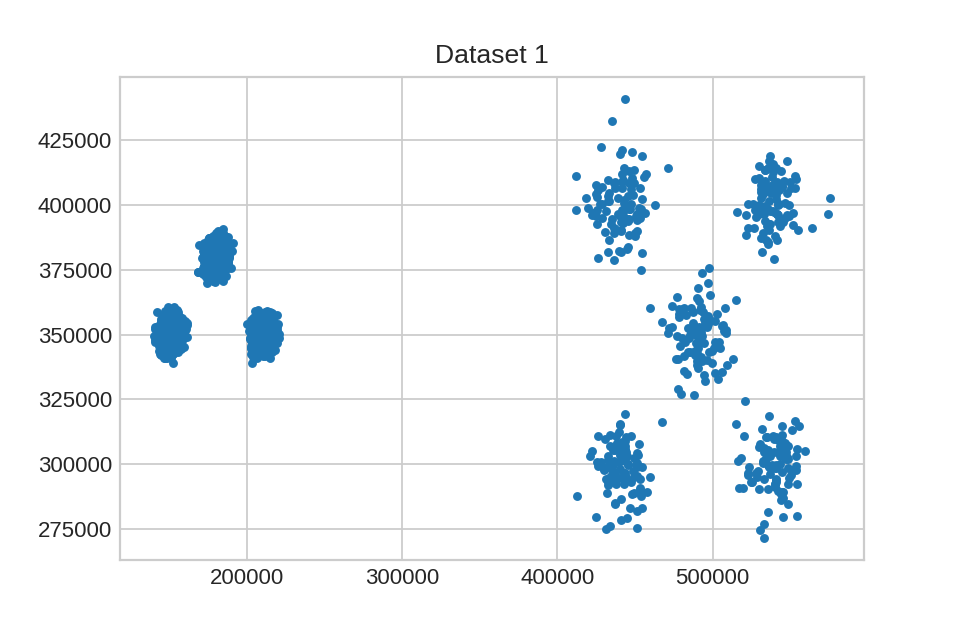
\includegraphics[scale=0.4]{experimentos/dataset1}
	\end{minipage}\qquad
	\begin{minipage}[t]{.3\textwidth}
		\centering
		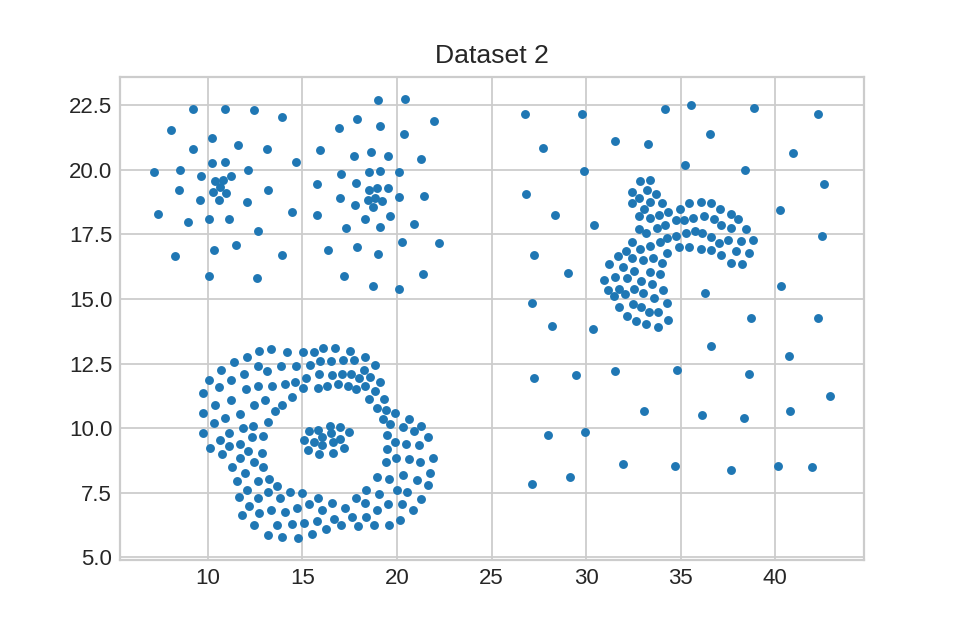
\includegraphics[scale=0.4]{experimentos/dataset2}
	\end{minipage}\qquad
	\begin{minipage}[t]{.3\textwidth}
		\centering
		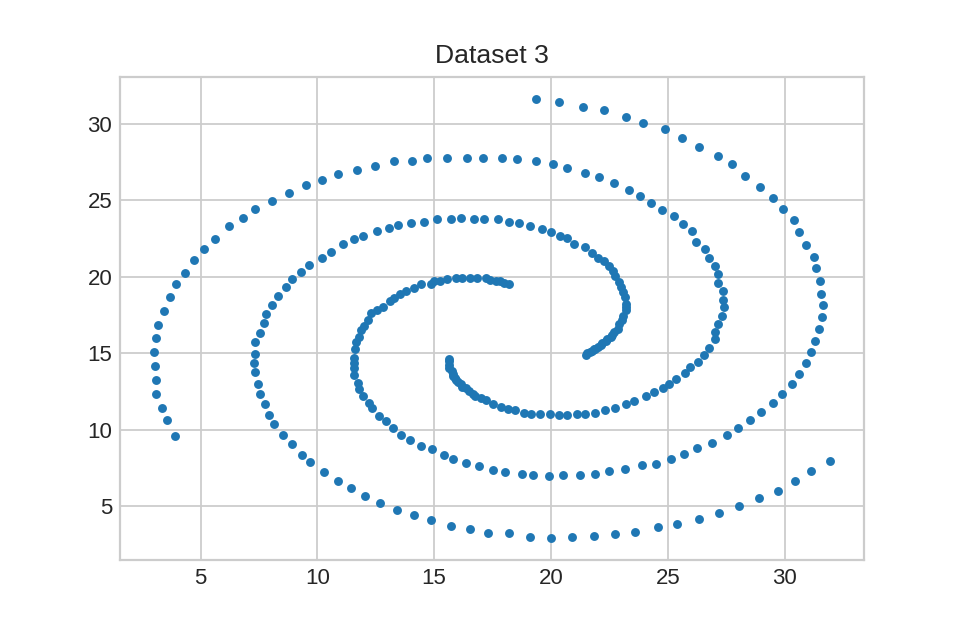
\includegraphics[scale=0.4]{experimentos/dataset3}
	\end{minipage}
\end{figure}	


\fbox{
	\parbox{0.9\textwidth}{
\textbf{Nota}: Para todos los criterios vamos a utilizar una profundidad de exploración fija de 9 ejes adyacentes. 
	}
}
\vspace{10 pt}

\subsubsubsection{Solo desvío estándar}
En este caso, vamos a descartar únicamente los ejes que son declarados inconsistentes al exceder en más de $\sigma$ veces el desvío estándar aplicado sobre el tamaño de eje promedio del vecindario.

\begin{figure}[H]
	\centering
	\begin{minipage}[t]{.3\textwidth}
		\centering
		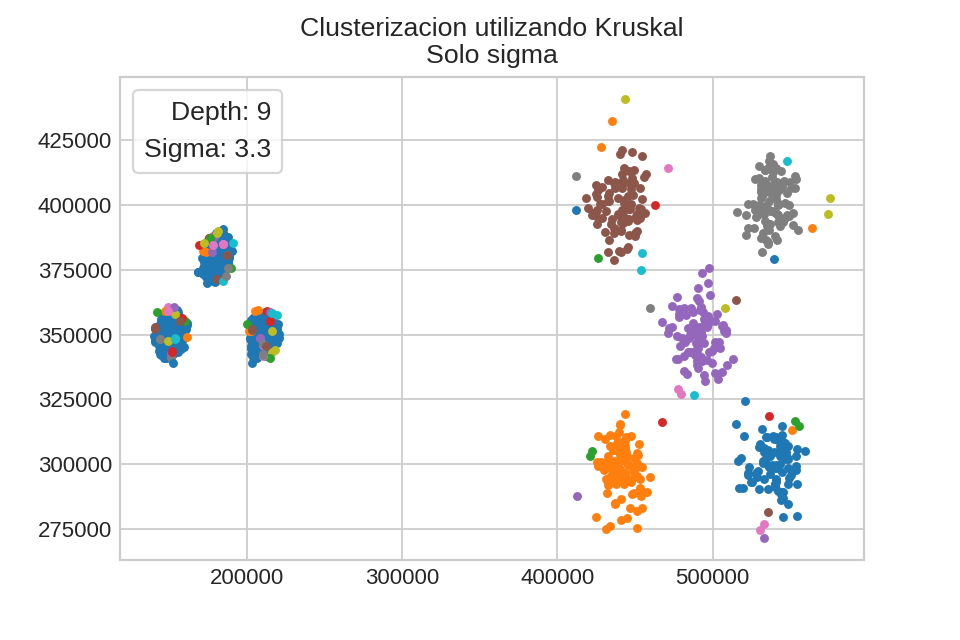
\includegraphics[scale=0.4]{experimentos/ds1-solosigma}
	\end{minipage}\qquad
	\begin{minipage}[t]{.3\textwidth}
		\centering
		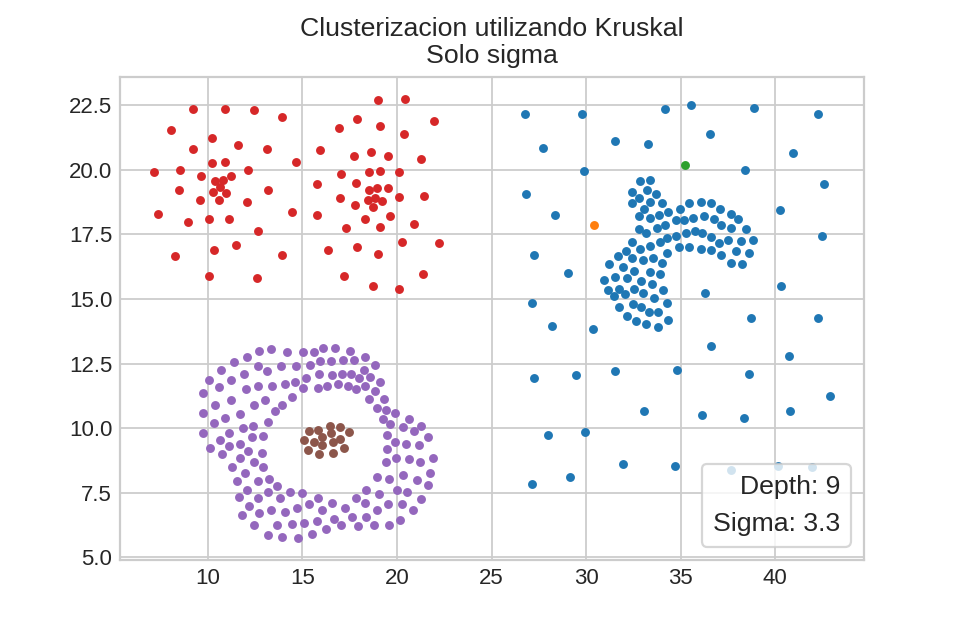
\includegraphics[scale=0.4]{experimentos/ds2-solosigma}
	\end{minipage}\qquad
	\begin{minipage}[t]{.3\textwidth}
		\centering
		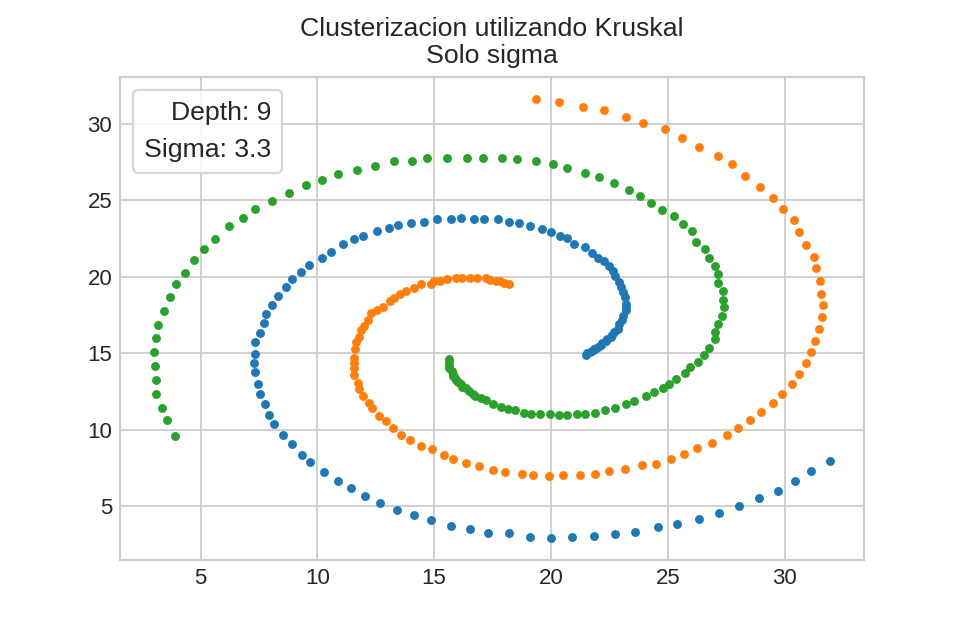
\includegraphics[scale=0.4]{experimentos/ds3-solosigma}
	\end{minipage}
\end{figure}	

Como podemos ver, utilizar solo el desvío estándar sirve para algunos casos, sin embargo tiene problemas para el \textit{dataset-1}, dado que en los clusters más chicos la desviación estándar entre los puntos es más alta, al estar todos más juntos. No podemos lograr un consenso de clusters sobre estos sin perjudicar la clusterización para los grupos de la derecha.


\subsubsubsection{Solo relación sobre el eje promedio}
En este caso, vamos a descartar únicamente los ejes que son declarados inconsistentes al ser $\digamma$ veces más grandes que el tamaño de eje promedio del vecindario.


\begin{figure}[H]
	\centering
	\begin{minipage}[t]{.3\textwidth}
		\centering
		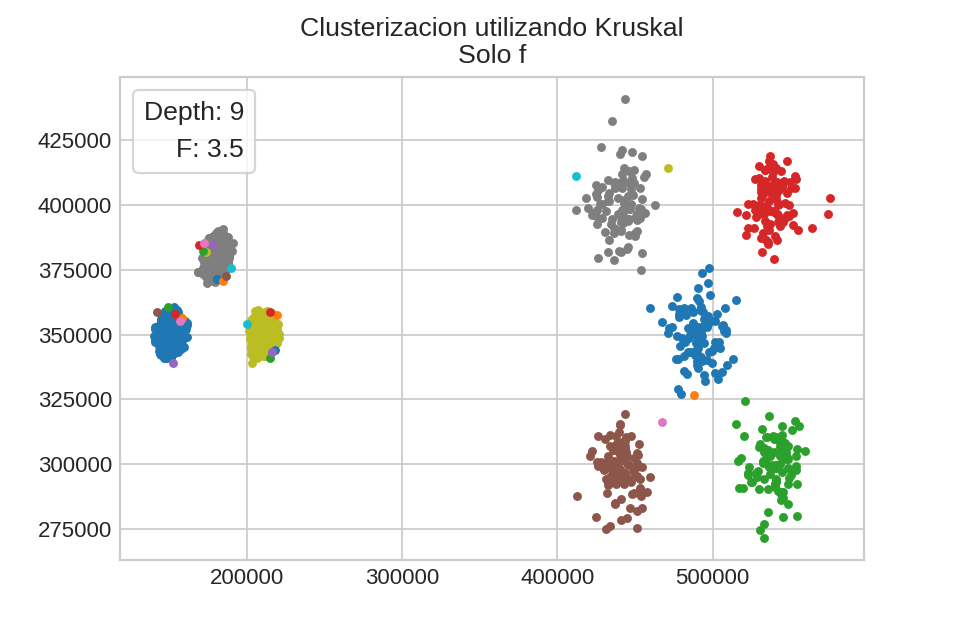
\includegraphics[scale=0.4]{experimentos/ds1-solof}
	\end{minipage}\qquad
	\begin{minipage}[t]{.3\textwidth}
		\centering
		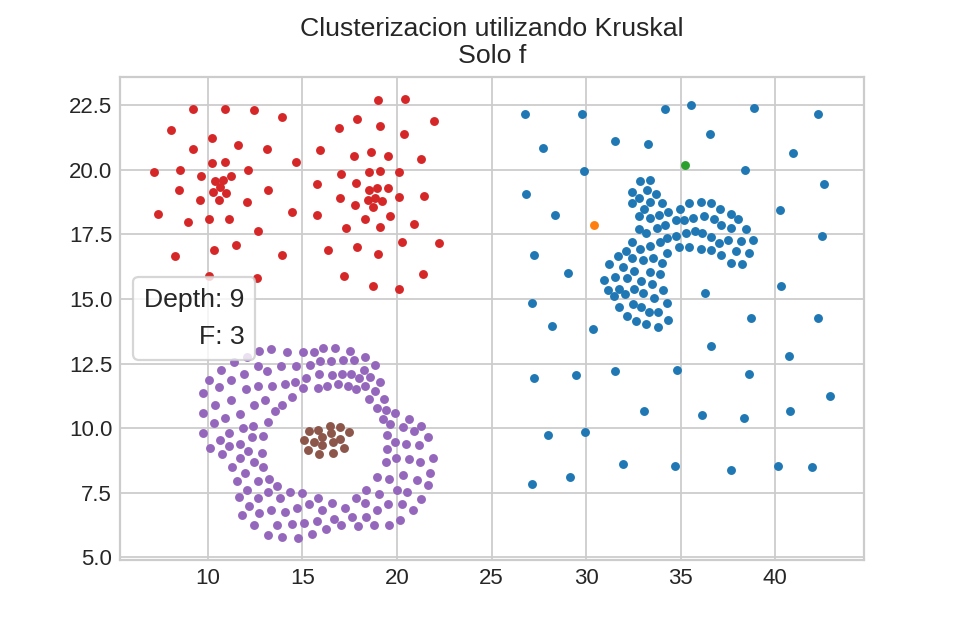
\includegraphics[scale=0.4]{experimentos/ds2-solof}
	\end{minipage}\qquad
	\begin{minipage}[t]{.3\textwidth}
		\centering
		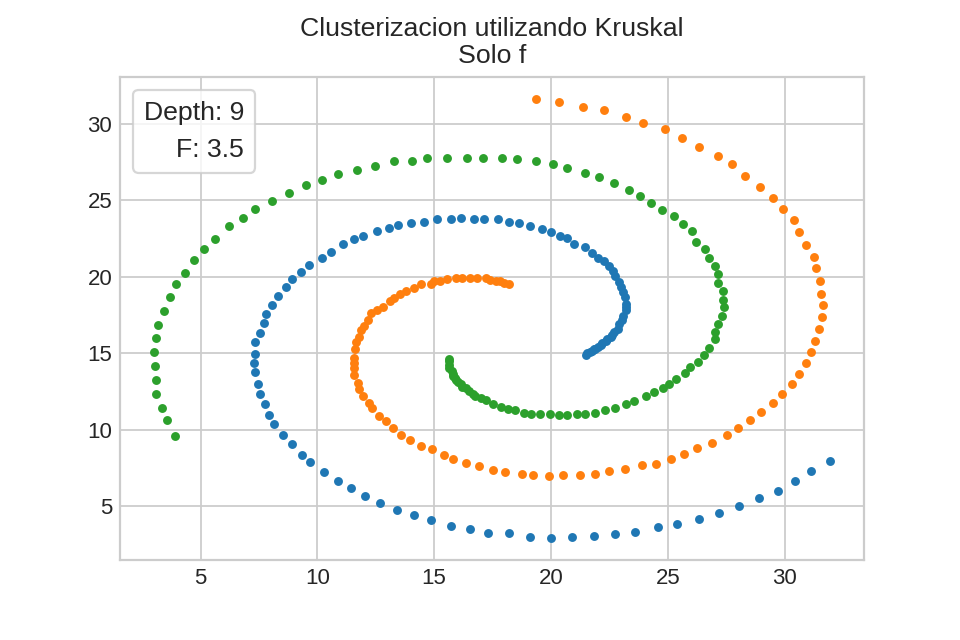
\includegraphics[scale=0.4]{experimentos/ds3-solof}
	\end{minipage}
\end{figure}

En este caso podemos ver que el \textit{dataset-1} no es problema para este criterio, aunque hay que notar que para el caso del \textit{dataset-2}, hubo que elegir un $f$ distinto, ya que los clusters de lado izquierdo eran agrupados con el valor utilizado para los otros datasets.

\subsubsubsection{Desvío estándar o relación de eje promedio}
Para este caso, los ejes inconsistentes van a ser los que cumplan con alguno de los dos criterios anteriores


\begin{figure}[H]
	\centering
	\begin{minipage}[t]{.3\textwidth}
		\centering
		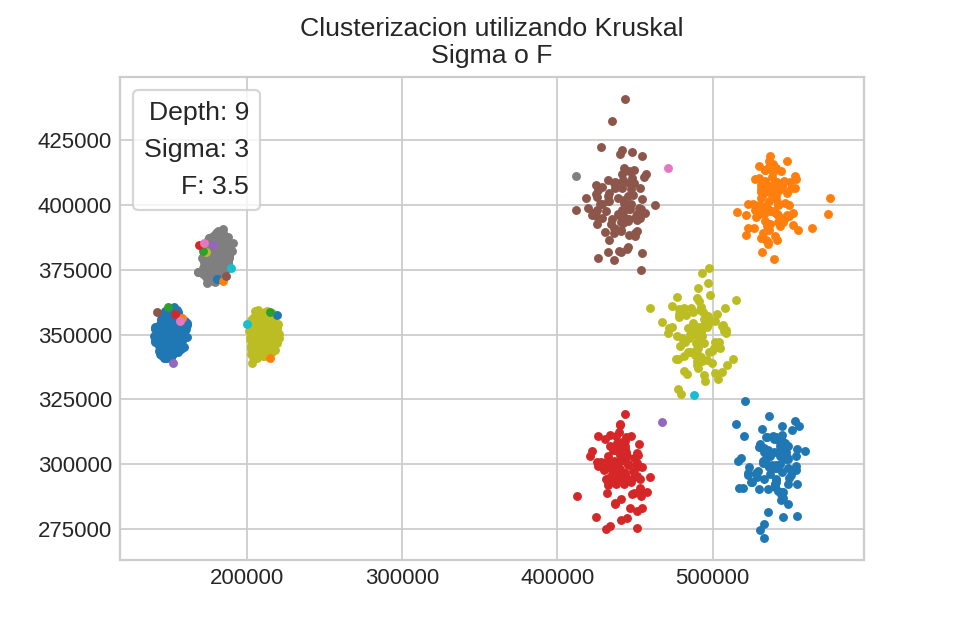
\includegraphics[scale=0.4]{experimentos/ds1-sigmaof}
	\end{minipage}\qquad
	\begin{minipage}[t]{.3\textwidth}
		\centering
		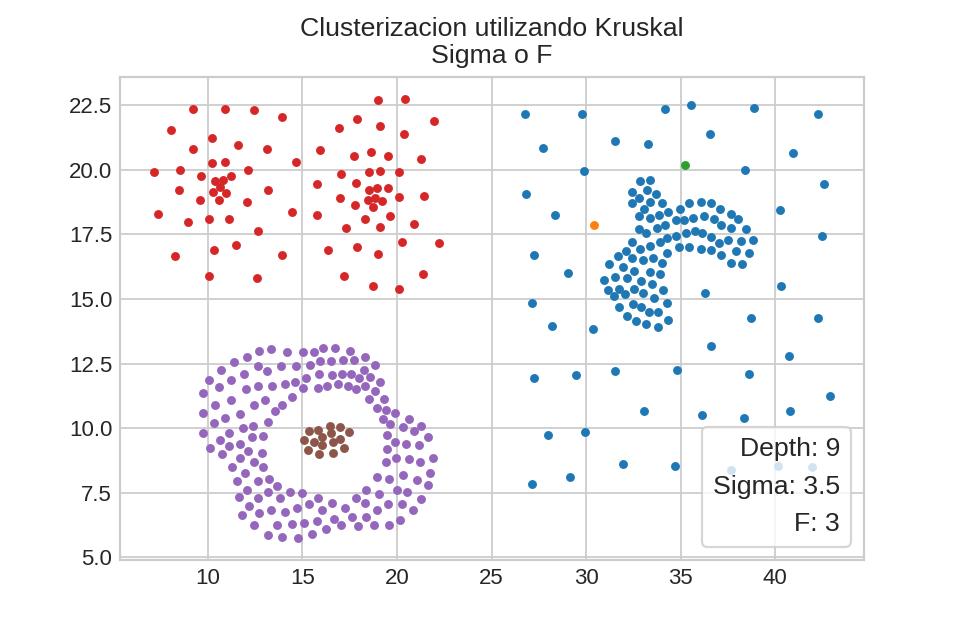
\includegraphics[scale=0.4]{experimentos/ds2-sigmaof}
	\end{minipage}\qquad
	\begin{minipage}[t]{.3\textwidth}
		\centering
		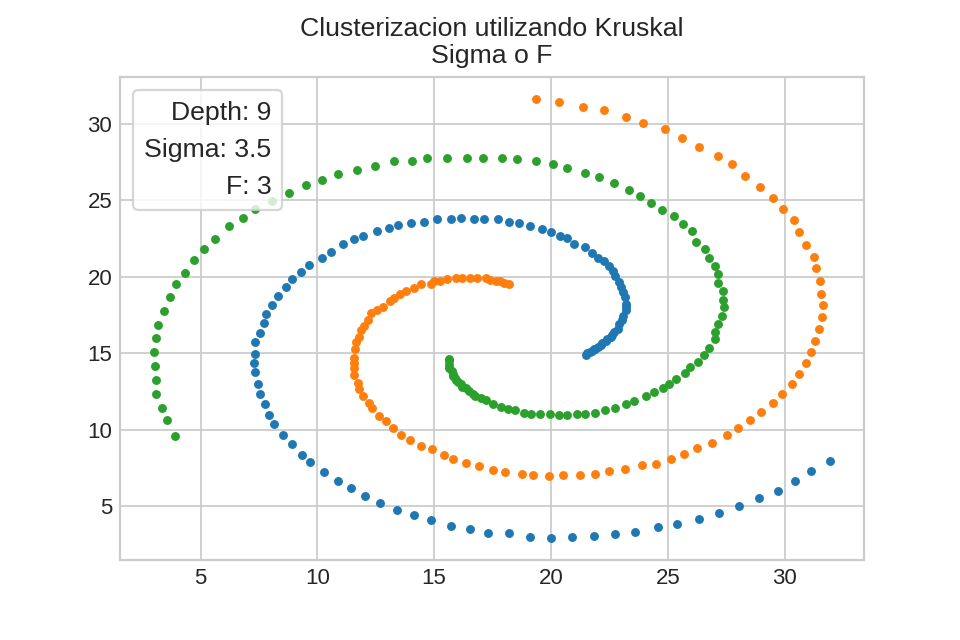
\includegraphics[scale=0.4]{experimentos/ds3-sigmaof}
	\end{minipage}
\end{figure}

Al utilizar cualquiera de los dos criterios anteriores para descartar nodos, podemos ver que en general toma precedencia el criterio por ‘f’ (relación de tamaño con el eje promedio). Por lo que no observamos beneficios al incluir el desvío estándar en la comparación. 

\subsubsubsection{Desvío estándar y relación de eje promedio}
Para este último caso, vamos a descartar únicamente los ejes que sean declarados inconsistentes tanto por el criterio del desvío estándar como por el criterio de relación de eje.

\begin{figure}[H]
	\centering
	\begin{minipage}[t]{.3\textwidth}
		\centering
		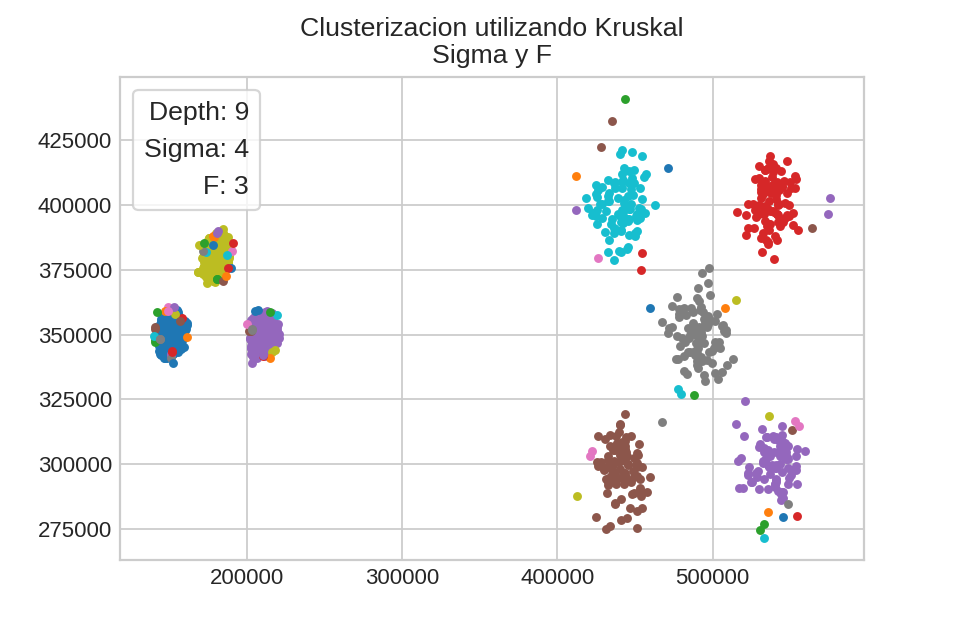
\includegraphics[scale=0.4]{experimentos/ds1-sigmayf}
	\end{minipage}\qquad
	\begin{minipage}[t]{.3\textwidth}
		\centering
		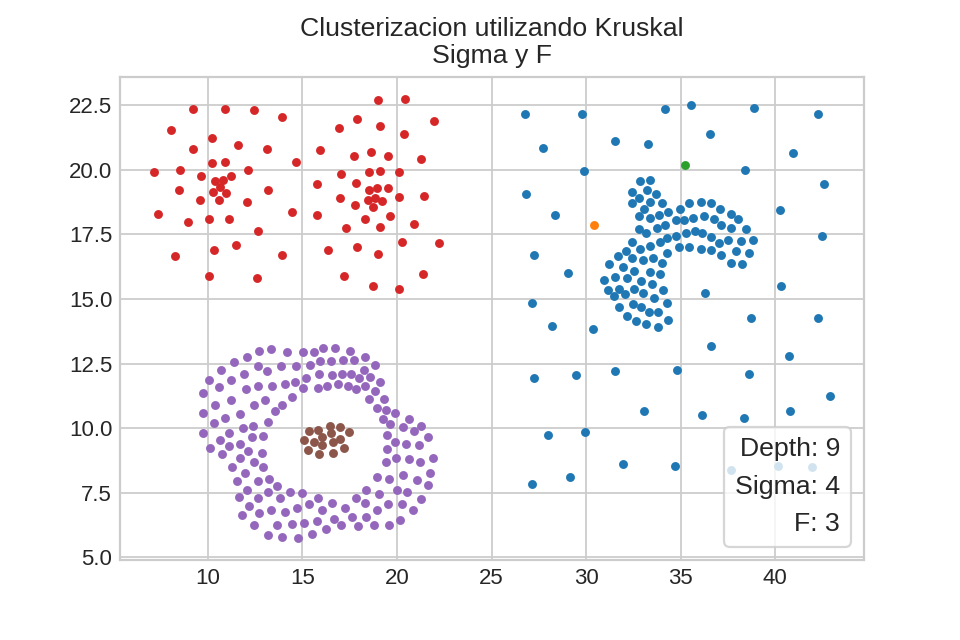
\includegraphics[scale=0.4]{experimentos/ds2-sigmayf}
	\end{minipage}\qquad
	\begin{minipage}[t]{.3\textwidth}
		\centering
		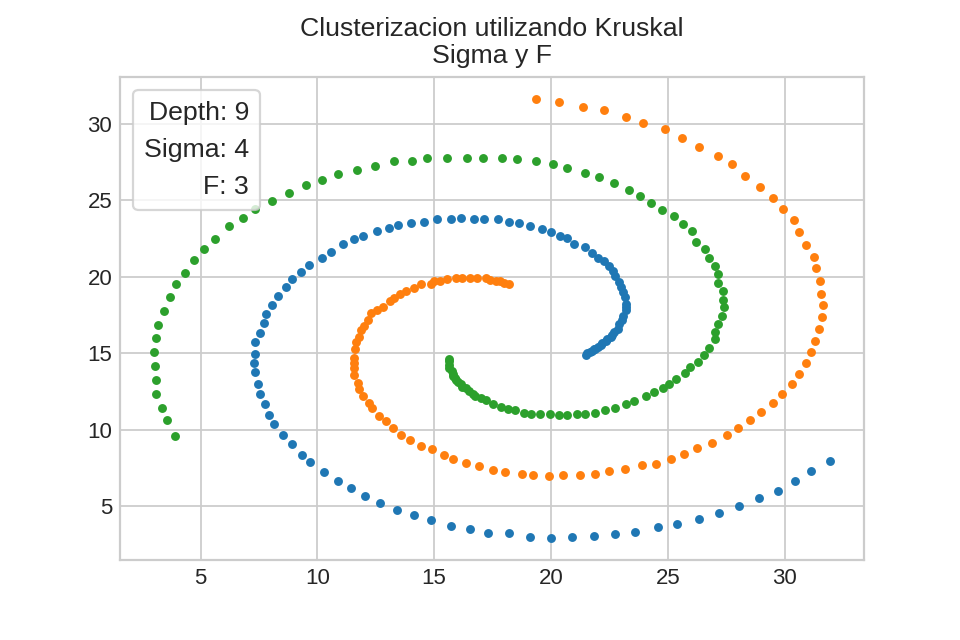
\includegraphics[scale=0.4]{experimentos/ds3-sigmayf}
	\end{minipage}
\end{figure}

Siguiendo el caso anterior, podemos ver que usar la conjunción sólo resulta en peores resultados, dado que para forzar la clusterización en algunos grupos, debemos usar un valor alto para sigma, lo cual resulta en agrupamientos indeseados en otras partes del grafo.

\subsubsubsection{Conclusiones}

Para los grafos elegidos para el experimento, resulta más conveniente utilizar únicamente la relación del eje contra el tamaño promedio de ejes. Como experimentos para profundizar, se deberían elegir grafos en los cuales la desviación estándar sea mayor al tamaño de eje promedio, en cuyo caso podríamos sacar provecho de combinar ambos criterios.

